\chapter{Рабочая среда разработчика встраиваемых систем}


\begin{itemize}
  \item Операционная система с набором типовых утилит
  
  Для Windows требуется дополнительно установить несколько модулей из пакета
  \file{GnuWin32}, чтобы обеспечить минимальную совместимость с UNIX-средой.
  Установка \file{GnuWin32}\ описана в \labref{winsoftinstall}.
  
  Установка Linux описана в \labref{debianinstall}.
  
  \item Система управления версиями (\term{VCS})
  
  VCS предназначены для хранения полной истории изменений файлов проекта, и
  позволяют получить выгрузку проекта на любой момент времени, вести несколько
  веток разработки, получить историю изменений конкретного файла, или сравнить
  две версии файла (\term{diff}).
  
  Установка VCS \git\ описана в \labref{gitinstall}.
  
  \item Текстовый редактор или интегрированная среда разработки (IDE)
  
  Редактирование текстов программ и скриптов сборки (компиляции) с
  цветовой подсветкой синтаксиса (в зависимости от языка файла),
  \term{автодополнением}\ и вызовом программ-утилит нажатием сочетаний 
  клавиш. Также включает различные вспомогательные функции, например
  отладочный интерфейс и отображение объектов программ.
  
  Установка IDE \eclipse\ описана в \labref{eclipseinstall}.
  
  \item Тулчайн
  
  Пакет кросс-компилятора, ассемблера, линкера и других утилит типа make,
  objdump,.. для получения прошивок из исходных текстов программ.
  
  Установка GNU toolchain описана в \labref{gnuinstall}.
  
  \item ПО для программатора, JTAG-адаптера
  
  Загрузка полученной прошивки в целевое устройство, редактирование памяти, 
  внутрисхемная отладка в процессе работы устройства, прямое измение сигналов на
  выводах процессора (граничное сканирование и тестирование железа).
  
  Установка ПО для адаптеров ST-Link \labref{stlinkinst}, Segger J-Link
  \labref{jlinkinst}.
  
  \item Симулятор для отладки программ без железа
  
  Симулятор может использоваться как ограниченная замена реального железа
  для начального обучения, и для отладки программ, не завязанных на работу
  железа.
  
  Установка QEMU \labref{qemuinstall}.
  
  \item Система верстки документации
  
  Для документирования проектов и написания руководств нужна система верстки
  документации, выполняющая трансляцию текстов программ и файлов 
  документации в выходной формат, чаще всего \file{.pdf} и \file{.html}.
  
  Установка \LaTeX\ \labref{texinstall}.
  
\end{itemize}



\labpart{Установка ПО}

\section{Выбор и установка операционной системы}

\subsection{MacOS}

Этот странный пока случай не рассматриваем\ --- у меня нет под рукой Мака \smiley.

\subsection{Windows}

Самый распространенный вариант. Вам придется ограничиться этим вариантом если вам не повезло
с поставщиком контроллера: windows-only ПО поддержки, например софт для программатора, или
внезапно библиотеки только для коммерческих компиляторов. Аналогичная ситуация будет в случае
покупки какого-нибудь специфичного оборудования (лог.анализатор, измерительное 
оборудование или просто принтер).

Установку ОС не рассматриваем.

\win{Секции текста книги, зависящие от ОС, будут выделены вот так.}

Для разработки встраиваемого ПО нужно поставить несколько пакетов, обеспечивающих
совместимость с UNIX средами \ref{winsoftinstall}.

\subsection{Linux}\label{linux}

\begin{enumerate}
\item \label{linuxref1}\linux\ удобен для разработчика, 
\item Если он вам не удобен, см п.\ref{linuxref1}
\end{enumerate}

\lin{Секции текста книги, зависящие от ОС, будут выделены вот так.}

\lin{\labwork{Установка Debian GNU/Linux}\label{debianinstall}}

\section{Установка инструментального программного обеспечения}

\win{\labwork{Установка инструментального ПО для Windows}\label{winsoftinstall}}

Создадим рабочий каталог, установим систему контроля версий \git\ref{git}\ и 
получим локальную копию проекта этой книги, содержащий кроме текста для издательской системы
\LaTeX\ еще и исходные коды библиотек, примеры кода и т.п., которые вы захотите
использовать в своих проектах.

%\labsection{Установка Git}\label{gitinstall}

\bigskip\wcmd{\url{http://git-scm.com/download/win}}

Запуститься закачка установочного пакета scm-git (\file{Git-1.9.4-preview20140611.exe}), после его загрузки
запустите установщик, 

\bigskip
\menu{Welcome>Next}

\bigskip
\menu{GNU GPL>Next} 

\bigskip
\menu{Select components>Windows Explorer Integration>Simple Context Menu>Git GUI here>Next}

\bigskip
\menu{Use Git and optional Unix tools from the Command Prompt>Next}

\bigskip
\menu{Use OpenSSH>Next}

\bigskip
\menu{Checkout Windows-style>Next}

\bigskip
\menu{Extracting files...}

\bigskip
\menu{Completing Setup>\uncheckbox\ View ReleaseNotes>Finish}

\bigskip
Проверим что \git\ правильно установился:

\bigskip\wcmd{cmd}

\bigskip
\begin{lstlisting}[style=con]
C:\Documents and Settings\pda>git --version
git version 1.9.4.msysgit.0
\end{lstlisting}

\bigskip
Первое, что вам следует сделать после установки \git а\ ---указать ваше имя и
адрес электронной почты. Это важно, потому что каждый коммит в \git е содержит
эту информацию, и она включена в коммиты, передаваемые вами:
\begin{lstlisting}[style=con]
C:\Documents and Settings\pda>git config --global user.name "Vasya Pupkin"
C:\Documents and Settings\pda>git config --global user.email no@mail.com
C:\Documents and Settings\pda>git config --global push.default simple
\end{lstlisting}

\bigskip
Эти настройки достаточно сделать только один раз, поскольку в этом случае 
\git\ будет использовать эти данные для всего, что вы делаете.
 Если для каких-то отдельных проектов вы хотите указать другое имя или
электронную почту, можно выполнить эту же команду без параметра \verb|--global|
в каталоге с нужным проектом.

\bigskip
Создаем каталог \directory{D:/ARM}\ и выгружаем текущую копию этой книги из репозитория
\url{https://github.com/ponyatov/CortexMx}

\bigskip\wcmd{cmd}

\bigskip
\begin{lstlisting}[style=con]
C:\Documents and Settings\ponyatov>D:
D:\>mkdir \ARM
D:\>cd \ARM
D:\ARM>git clone --depth=1 https://github.com/ponyatov/CortexMx.git book
\end{lstlisting}



\lin{\labwork{Установка инструментального ПО для \linux}\label{linsoftinstall}}

\chapter{Управление версиями при написании ПО}

\section{Git}\label{git}\cite{progit}


\section{Общая структура рабочей среды разработчика встроенных систем}

\begin{itemize}
  \item Операционная система с набором типовых утилит
  
  Для Windows требуется дополнительно установить несколько модулей из пакета
  \file{GnuWin32}, чтобы обеспечить минимальную совместимость с UNIX-средой.
  Установка \file{GnuWin32}\ описана в \labref{winsoftinstall}.
  
  Установка Linux описана в \labref{debianinstall}.
  
  \item Система управления версиями (\term{VCS})
  
  Рекомендую использовать \git\ и один из проектных хостингов типа
  \url{https://github.com/}. Установка описана в \labref{winsoftinstall}.
  
  VCS предназначены для хранения полной истории изменений файлов проекта, и
  позволяют получить выгрузку проекта на любой момент времени, вести несколько
  веток разработки, получить историю изменений конкретного файла, или сравнить
  две версии файла (\term{diff}).
  
  Избегайте использования бинарных файлов, по возможности генерируйте их из
  текстового описания на каком-нибудь макроязыке\ --- в этом случае VCS
  обеспечит вам возможность получить историю или diff в
  человекочитаемопонимаемом виде, а не в виде набора невнятных кексов.
  
  \item Текстовый редактор или интегрированная среда разработки (IDE)
  
  Редактирование текстов программ и скриптов сборки (компиляции) с
  цветовой подсветкой синтаксиса (в зависимости от языка файла),
  \term{автодополнением}\ и вызовом программ-утилит нажатием сочетаний 
  клавиш. Например нажатием \keys{F3}\ в \eclipse\ можно переместится на
  определение функции, на имени которой находится текствый курсор.
  
  Автодополнение\ --- редактор предлагает варианты полного написания
  идентификаторов и ключевых слов по первым буквам и нажатию обычно
  \keys{Ctrl+Tab} или \keys{Ctrl+N}. Также автоматически расставляются
  закрывающие скобки, закрывающие операторы управляющих структур типа begin/end,
  и генерируются синтаксические элементы циклов при вводе ключевых слов
  if/for/while. Особенно удобно автодополнение при написании кода на ООП 
  языках\  --- при вводе имени класса или объекта и точки предлагается меню с
  именами данных и методов класса. 
  
  При вводе имени функции и скобки выводится всплывающее окно с подсказкой\ ---
  определение функции с типом возвращаемого значения, типом и именами
  параметров.
  
  Интерфейс IDE часто предусматривает различные вспомогательные окна,
  показывающие имена и свойства объектов, описанных в программе (переменные,
  функции, структуры,..), структуру проекта с зависимостями между файлами, блоки
  справки в зависимости от текущего выделенного элемента и т.п.
  
  Часто IDE имеет встроенный графический интерфейс для отладки программ,
  используя для этого интерфейсные библиотеки для программатора и
  специальный отладочный код, добавляемый к вашей программе при
  компиляции. Используя аппаратный модуль отладки на целевом процессоре и
  отладочный код, IDE обеспечивает отображение значений и изменений регистров
  процессора, состояние переферии, позволяет задать точки останова в программном
  коде, в т.ч. условные по значению или измениею переменных или регистров
  железа.
  При использовании ОС реального времени и системы аппаратной многозадачности
  отображается загрузка ядер, загрузка процессора и используемые ресурсы для
  каждой задачи, работа планировщика, и т.п.
  
  \item Пакет кросс-компилятора и утилит типа make, objdump,..
  
  Компилятор преобразует программы на языке программирования в \term{объектный
  код} (смесь кусочков машинного кода со служебной информацией) или в
  текст на языке ассемблера.
  
  \term{Кросс-компилятор}\ (arm-none-eabi-gcc) отличается от обычного
  компилятора тем, что генерирует код не для компьютера на котором он выполняется
  (\term{хост-система}, \verb|$HOST|), а для компьютера другой
  архитектуры\ --- \term{целевой} системы, \verb|$TARGET|.
  
  \term{Ассемблер}\ (as) преобразует человекочитаемый код программы в объектный
  код.
  
  \term{Линкер}\ (ld) объединяет несколько файлов объектного кода в один,
  и корректирует машинный код с учетом его конечного размещения в памяти
  целевой системы (адреса переменных, адреса переходов, размещение сегментов
  кода и данных в физической памяти целевой системы).
  
  \term{Дампер}\ (objdump) преобразует сегменты кода/данных из файла,
  полученного линкером, в формат, необходимый для ПО программатора: бинарные файлы, Intel
  HEX, ELF,.. загружаемые в масочное ПЗУ, FlashPROM (и EEPROM данных на МК
  ATmega).
  
  \item ПО для программатора, JTAG-адаптера
  
  Загрузка полученной прошивки в целевое устройство, редактирование памяти, 
  внутрисхемная отладка в процессе работы устройства, прямое измение сигналов на
  выводах процессора (граничное сканирование и тестирование железа).
  
  \item Система верстки документации
  
  Для документирования проектов и написания руководств нужна система верстки
  документации, выполняющая трансляцию текстов программ и файлов 
  документации в выходной формат, чаще всего \file{.pdf} и \file{.html}.
  
  Необходимо использовать человеко-читаемые простые текстовые файлы 
  (\file{plain ascii text}, кодировка по выбору, удобнее всего \file{utf8}) и
  использовать язык разметки\ --- DocBook, а удобнее всего \LaTeX.
  
  \alarm{
  Ни в коем случае не используйте для документации всякую бинарщину тип
  NarcoSoft Word\ --- текстовый формат необходим для корректной 
  и полноценной работы VCS. 
  Исключение по необходимости\ --- только графические файлы, подключаемые
  при генерации выходных файлов документации.
  }
  
  Эта книга написана с использованием языка разметки \LaTeX, и транслируется
  в экранный \file{.pdf} с помощью пакета \win{MiKTeX}/\lin{TeXlive}.
  
  Установка опиасана в \labref{instex}
  
\end{itemize}

\win{\labwork{Установка IDE}\label{winide}}

Для удобной работы доступно несколько бесплатных вариантов IDE (интегрированных сред разработки),
рассмотрим два варианта: тяжелая суперуниверсальная среда Eclipse, и легкая в отношении требуемых
ресурсов системы CodeLite.

\bigskip Для работы Eclipse требуется установленная Java:

\bigskip\wcmd{\url{http://www.oracle.com/technetwork/java/javase/downloads/}}

\bigskip\begin{itemize}
  \item 
Минимальный вариант\ ---  ставим только Java Runtime:

\menu{Java Platform, Standard Edition>JRE>Download>Accept
License>\file{jre-8u5-windows-i586.exe}}

\menu{\file{jre-8u5-windows-i586.exe}>Welcome>\checkbox\ Change destination
folder>Install}

\menu{Destination folder>\file{D:/Java/jre8}>Next>Installing>Close}

  \item
Если вы планируете параллельно еще и осваивать язык Java\ --- ставим
Java SE JDK: 

\menu{Java Platform, Standard Edition>JDK>Download>Accept
License>\file{jdk-8u5-windows-i586.exe}}

\menu{\file{jdk-8u5-windows-i586.exe}>Welcome>Next}

\menu{Install to: \file{D:/Java/jdk8}>Next}

\menu{JRE Distination folder>Install to: \file{D:/Java/jre8}>Next}

\menu{Java SE Development Kit 8 Update 5 Successfully Installed>Close}

\end{itemize}

Для установки доступны два варианта:
\begin{enumerate}
\item \textbf{Eclipse Standard} базовый вариант среды, в ЛР рассмотрен именно он для иллюстрации 
ручной установки расширений
\item \textbf{Eclipse IDE for C/C++ Developers} вариант сборки 
уже включает расширение CDT, поэтому в следующий раз рекомендуем сразу качать его,
это упростит и съэкономит немного времени на установку рабочей среды
\end{enumerate}

\bigskip\wcmd{\url{http://www.eclipse.org/downloads/}}

\bigskip\menu{Eclipse Standard>Windows 32
Bit>Download>\file{eclipse-standard-luna-R-win32.zip}}

\bigskip Перетащите каталог \file{eclipse} из архива в \file{D:/ARM} и
создайте удобным для вас способом ссылку на \file{D:/ARM/eclipse/eclipse.exe}.

\bigskip
\includegraphics[height=0.3\textheight]{fig/EclipseSplash.png}

\bigskip Workspace\ --- рабочий каталог, в котором создаются каталоги отдельных
проектов, типа \file{D:/WORK}. Eclipse создаст в нем служебный каталог
\file{.metadata}, и поместит в него служебную информацию, относящуюся сразу ко
всем проектам. Как побочный эффект, если в workspace уже есть какой-то каталог,
можно создать новый проект (например \file{book}), и в левой части рабочей
области \eclipse\ в окне \window{Project Explorer}\ появится дерево файлов
\file{book/*}.

\bigskip\menu{\file{D:/ARM/eclipse/eclipse.exe}>Workspace>\file{D:/ARM}>Use as
default>OK}

\bigskip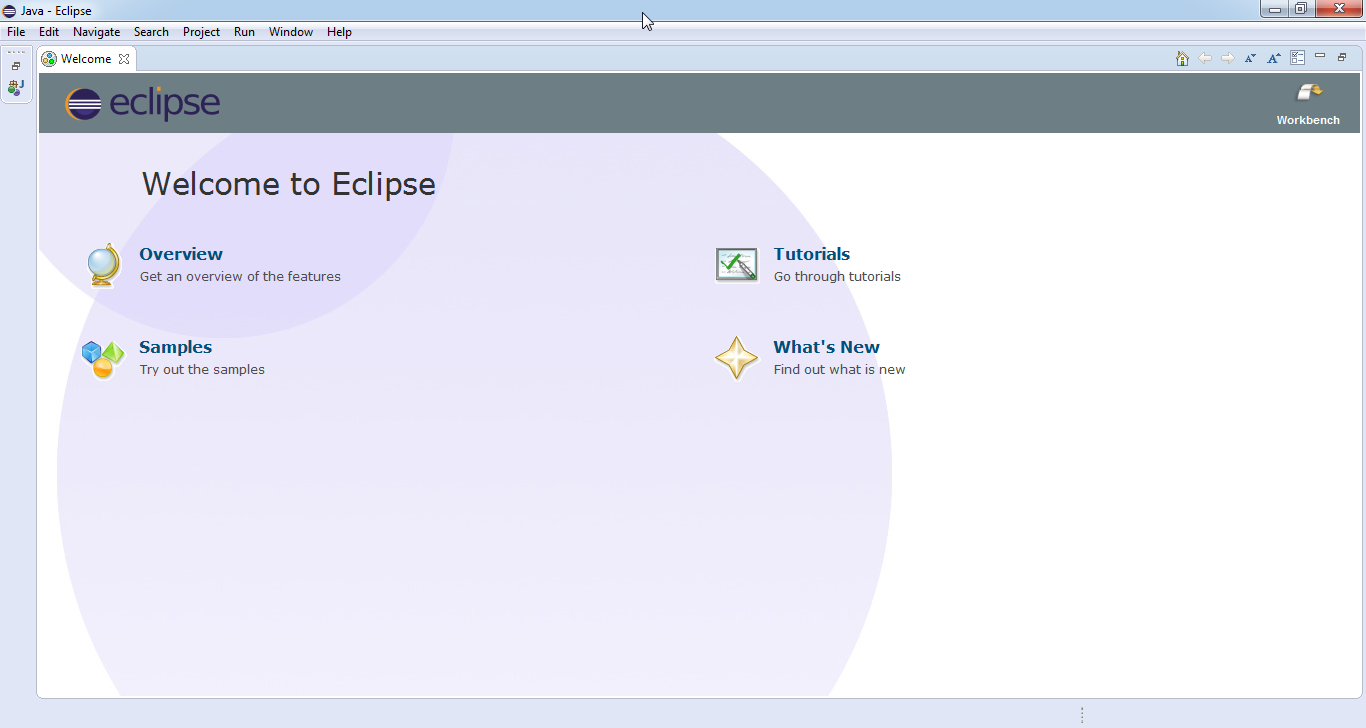
\includegraphics[width=0.9\textwidth]{fig/EclipseMain.png}

\bigskip Проверяем наличие обновлений

\bigskip\menu{Help>Check for Updates>Details>No updates found>OK}

\bigskip В базовом варианте Eclipse поддерживает только Java, поэтому нужно
установить расширение для работы с С/C++: \file{CDT}.

\bigskip
Проект \file{CDT}\ предоставляет полнофункциональную интегрированную среду
для разработки на Си и \cpp. Поддерживаются: управление проектами и
компиляцией для различных тулчейнов, стандартная сборка через
\file{make}, навигация по исходным текстам, различные инструменты для
работы с иходным текстом, такие как иерархия типов, граф вызовов, браузер
подключаемых файлов, браузер макроопределений, редактор кода с подсветкой
синтаксиса, сворачивание синтаксических структур (фолдинг) и гипертекстовая
навигация, рефакторинг и генерация кода, средства визуальной отладки,
включающие просмотр памяти, регистров и дизассемблер.

\bigskip\wcmd{\url{http://www.eclipse.org/cdt/downloads.php}}

\bigskip Выделить и скопировать в буфер обмена ссылку

\file{p2 software repository}:
\url{http://download.eclipse.org/tools/cdt/releases/8.4}.

\bigskip Добавляем сетевое хранилище пакетов для \eclipse:

\bigskip\menu{\eclipse>Help>Install New Software>Work with>Add}

\bigskip\menu{Name>CDT}

\menu{Location>http://download.eclipse.org/tools/cdt/releases/8.4}

\menu{OK}

\bigskip
Выбрать (если оно не выбралось само) хранилище \menu{Work with:>CDT},
и в дереве выбора пакетов выбрать:

\bigskip
\dirtree{%
.1 CDT.
.2 CDT Main Features.
.3 \checkbox\ C/C++ Development Tools.
.2 CDT Optional Features.
.3 \checkbox\ C/C++ C99 LR Parser.
.3 \checkbox\ C/C++ GCC Cross Compiler Support.
.3 \checkbox\ C/C++ GDB Hardware Debugging.
}

\bigskip
\menu{Next>Next>Licenses>Accept>Finish}

\bigskip После установки пакетов появится окно с запросом перезапуска \eclipse.

\bigskip Аналогично ставим плагин GNU ARM Eclipse:

\bigskip
\menu{Help>Install>Work with>Add}

\menu{Name>GNU ARM plugin}

\menu{Location>\url{http://sourceforge.net/projects/gnuarmeclipse/files/Eclipse/updates/}}

\dirtree{%}
.1 GNU ARM C/C++ Cross Development Tools.
.2 \checkbox\ Cross Compiler Support.
.2 \checkbox\ Generic Cortex-M Project Template.
.2 \checkbox\ STM32Fx Project Templates.
.2 \checkbox\ OpenOCD Debugging Support.
}

\menu{Warning: You install unsigned content>Ok}

\bigskip
В \eclipse\ есть так называемые \term{перспективы} (perspective)\ --- это
переключаемые режимы отображения рабочего набора окон, настроенные под тип
работы. По умолчанию запускается перспектива \window{Java}. Нас
интересует перспектива \window{C/C++}:

\bigskip\menu{Window>Open Perspective>Other>C/C++>Ok}

\bigskip Также перспективу можно переключить кнопкой на панели в правом верхнем
углу:

\bigskip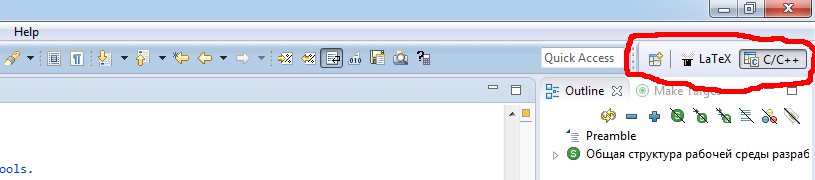
\includegraphics[width=0.9\textwidth]{fig/eclperpective.png}

\labwork{Установка системы верстки документации \LaTeX}\label{instex}

\bigskip
\menu{\eclipse>Help>Install>Work with>Add}

\menu{Name>TeXlipse}

\menu{Location>\url{http://texlipse.sourceforge.net}}

\dirtree{%}
.1 TeXlipse.
.2 \checkbox\ TeXlipse.
}
